In questo capitolo verranno analizzati tre aspetti principali:
\begin{itemize}
	\item Cos'è un \textbf{canale di trasmissione}, come viene modellato nella teoria della comunicazione e come viene utilizzato in modo efficace tramite \textbf{codifica} e \textbf{modulazione}.
	\item Come un canale di trasmissione può essere condiviso tra più utenti tramite tecniche di \textbf{multiplazione} e \textbf{accesso multiplo}.
	\item Quali sono i \textbf{mezzi fisici} utilizzati per creare canali di trasmissione.
\end{itemize}
\section{Introduzione alla teoria della comunicazione}
In generale il modello adottato è quello proposto da Shannon e Weaver, 
che rappresenta la comunicazione come un processo in cui un \textbf{mittente} invia un \textbf{messaggio} attraverso un \textbf{canale di trasmissione} a un \textbf{destinatario}.
Il canale di trasmissione è soggetto a \textbf{rumore}, che può distorcere o degradare il messaggio durante la trasmissione. 

\begin{figure}[htbp]
\centering
\resizebox{\textwidth}{!}{%
\begin{tikzpicture}[
		>=Stealth,
	font=\footnotesize,
		block/.style={draw, thick, minimum width=3.0cm, minimum height=1.6cm, align=center, font=\bfseries},
		smallblock/.style={draw, thick, minimum width=2.8cm, minimum height=1.6cm, align=center, font=\bfseries},
	lab/.style={font=\normalfont\footnotesize}
]

% Main chain
\node[block] (src) at (0,0) {Information\\Source};
\node[block] (tx)  at (4.2,0) {Transmitter\\(Encoder)};
\node[block] (ch)  at (8.4,0) {Transmission\\Channel};
\node[block] (rx)  at (12.6,0) {Receiver\\(Decoder)};
\node[block] (dst) at (16.8,0) {Destination};

% Forward arrows + labels
\draw[->, thick] (src) -- node[above=1pt, lab] {Message} (tx);
\draw[->, thick] (tx) -- node[above=1pt, lab] {Signal} (ch);
\draw[->, thick] (ch) -- node[above=1pt, lab, align=center] {Received\\Signal} (rx);
\draw[->, thick] (rx) -- node[above=1pt, lab, align=center] {Received\\Message} (dst);

% Noise source and upward arrow
\node[smallblock] (noise) at (8.4,-3.0) {Noise\\Source};
\draw[->, thick] (noise.north) -- (ch.south);

% Braces under transmitter and receiver
\draw[decorate, decoration={brace, mirror, amplitude=7pt}, thick]
	([yshift=-0.45cm]tx.south west) -- ([yshift=-0.45cm]tx.south east)
	node[midway, below=0.85cm, align=center, font=\itshape\normalfont] {Coding and\\modulation};

\draw[decorate, decoration={brace, mirror, amplitude=7pt}, thick]
	([yshift=-0.45cm]rx.south west) -- ([yshift=-0.45cm]rx.south east)
	node[midway, below=0.85cm, align=center, font=\itshape\normalfont] {Demodulation\\and decoding};

% Transmission medium arrow (below noise source)
\draw[<->, thick]
	(2.8,-5.0) -- node[above, font=\bfseries] {Transmission medium} (14.0,-5.0);

\end{tikzpicture}%
}
\caption{Communication system block diagram}
\end{figure}
L'aggiunta del rumore modella il fallimento della comunicazione.

\subsection{Canale di trasmissione e capacità}
Nel seguito consideriamo principalmente comunicazioni digitali. Il canale può essere visto come un modello composto da:
\begin{itemize}
\item una funzione di trasferimento del canale $h_C(t)$, che rappresenta attenuazione e distorsione;
\item un termine di rumore $n(t)$, che degrada il segnale ricevuto.
\end{itemize}
La capacità di un canale è la massima velocità di trasmissione di informazione (in bit/s) che può essere raggiunta con un tasso di errore arbitrariamente basso, cioè in maniera "affidabile".
La capacità teorica massima di un canale rumoroso è data dalla formula di Shannon:
\[
C = B\,\log_2\!\left(1 + \frac{S}{N}\right) \quad [\text{bit/s}]
\]
dove $B$ è la banda del canale, $S$ la potenza del segnale e $N$ la potenza di rumore.
Nota che $B$ è fissato, quindi il rapporto segnale rumore definisce la capacità massima raggiungibile. Per avvicinarsi a questa capacità è necessario progettare codici di sorgente e di canale efficienti, oltre a modulazioni che sfruttino al meglio le caratteristiche del canale.
\subsection{Modulazione e codifica}
\begin{itemize}
\item \textbf{Modulazione analogica}: traslazione in frequenza di un segnale modulante su una portante. Dunque si aumenta la frequenza del segnale, viene effettuata cambiando ampiezza, frequenza o fase della portante.
\item \textbf{Modulazione digitale}: associazione di forme d'onda (simboli) a gruppi di bit in modo da ottenere un segnale robusto rispetto distorsioni e rumore.
	Ogni forma d'onda rappresenta un simbolo e dura per un certo periodo. Il numero di simboli trasmessi al secondo è detto \textbf{baud rate}.

\item \textbf{Codifica di sorgente}: compressione dell'informazione (loss-less e lossy).
\item \textbf{Codifica di canale}: aggiunta controllata di ridondanza per rilevare/correggere errori.
\end{itemize}

\section{Multiplazione}
La multiplazione permette di condividere la capacità di un canale tra più flussi informativi, tipicamente dividendo una risorsa (frequenza, tempo, codice).

\begin{figure}[htbp]
\centering
\begin{tikzpicture}[
	>=Stealth,
	font=\footnotesize,
	box/.style={draw, thick, align=center, minimum width=3.2cm, minimum height=0.9cm},
	arrow/.style={->, thick}
]
\node[box, font=\bfseries] (mux) at (0,0) {Multiplazione};

\node[box] (fdm) at (-5.1,-1.8) {Divisione in frequenza\\FDM / OFDM / WDM};
\node[box] (tdm) at (0,-1.8) {Divisione nel tempo\\TDM sincrona / asincrona};
\node[box] (cdm) at (5.1,-1.8) {Divisione per codice\\CDM};

\draw[arrow] (mux) -- (fdm);
\draw[arrow] (mux) -- (tdm);
\draw[arrow] (mux) -- (cdm);

\node[box] (sync) at (-1.8,-3.6) {Sincrona \\(slot periodici)};
\node[box] (async) at (1.8,-3.6) {Asincrona \\(pacchetti)};
\draw[arrow] (tdm) -- (sync);
\draw[arrow] (tdm) -- (async);
\node[box](slotted) at (0,-5.4) {slotted};
\draw[arrow] (async) -- (slotted);
\node[box] (unslotted) at (3.6,-5.4) {unslotted};
\draw[arrow] (async) -- (unslotted);

\end{tikzpicture}
\caption{Tassonomia semplificata delle tecniche di multiplazione}
\end{figure}\noindent
Nelle reti reali la multiplazione è spesso \textbf{gerarchica}: l'uscita di un multiplexer può essere a sua volta ingresso di un multiplexer di livello superiore.
\begin{figure}[H]
\centering
\begin{tikzpicture}[
	>=Stealth,
	font=\footnotesize,
	box/.style={draw, thick, align=center, minimum width=2.6cm, minimum height=0.85cm},
	arrow/.style={->, thick}
]
\node[box] (s1) at (0,1.2) {Sorgente 1};
\node[box] (s2) at (0,0) {Sorgente 2};
\node[box] (s3) at (0,-1.2) {Sorgente 3};

\node[box, minimum width=2.2cm, font=\bfseries] (m1) at (3.8,0.6) {MUX 1};
\node[box, minimum width=2.2cm, font=\bfseries] (m2) at (3.8,-0.9) {MUX 2};

\node[box, minimum width=2.5cm, font=\bfseries] (m3) at (7.6,-0.15) {MUX livello 2};
\node[box, minimum width=3.2cm] (out) at (11.4,-0.15) {Canale multiplato};

\draw[arrow] (s1) -- (m1);
\draw[arrow] (s2) -- (m1);
\draw[arrow] (s3) -- (m2);
\draw[arrow] (s2) -- (m2);
\draw[arrow] (m1) -- (m3);
\draw[arrow] (m2) -- (m3);
\draw[arrow] (m3) -- (out);
\end{tikzpicture}
\caption{Esempio di gerarchia di multiplazione}
\end{figure}

\subsection{Frequency Division Multiplexing (FDM)}
Nella multiplazione a divisione di frequenza, ogni flusso occupa una sotto-banda distinta.

\begin{figure}[H]
\centering
\resizebox{\textwidth}{!}{%
\begin{tikzpicture}[font=\footnotesize, >=Stealth, line join=round]

% --- Colori ---
\colorlet{specfill}{yellow!40}
\colorlet{chanfill}{red!10}

% --- Spettri in ingresso (sinistra) ---
% Ingresso 1
\draw[->] (0.2,5.6) -- (0.2,7.6);
\draw[->] (0.2,5.6) -- (2.8,5.6) node[right] {$f$};
\filldraw[fill=specfill, draw=black, thick]
	(0.55,5.6) .. controls (0.7,6.1) and (0.75,6.8) .. (0.75,7.1)
	.. controls (0.75,7.45) and (1.65,7.45) .. (1.65,7.1)
	.. controls (1.65,6.8) and (1.72,6.1) .. (1.82,5.6) -- cycle;
\node at (1.2,6.35) {1};
\node at (1.75,5.2) {$f_c$};

% Ingresso 2
\draw[->] (0.2,3.0) -- (0.2,5.0);
\draw[->] (0.2,3.0) -- (2.8,3.0) node[right] {$f$};
\filldraw[fill=specfill, draw=black, thick]
	(0.55,3.0) .. controls (0.7,3.5) and (0.75,4.2) .. (0.75,4.5)
	.. controls (0.75,4.85) and (1.65,4.85) .. (1.65,4.5)
	.. controls (1.65,4.2) and (1.72,3.5) .. (1.82,3.0) -- cycle;
\node at (1.2,3.75) {2};
\node at (1.75,2.6) {$f_c$};

% Ingresso 3
\draw[->] (0.2,0.4) -- (0.2,2.4);
\draw[->] (0.2,0.4) -- (2.8,0.4) node[right] {$f$};
\filldraw[fill=specfill, draw=black, thick]
	(0.55,0.4) .. controls (0.7,0.9) and (0.75,1.6) .. (0.75,1.9)
	.. controls (0.75,2.25) and (1.65,2.25) .. (1.65,1.9)
	.. controls (1.65,1.6) and (1.72,0.9) .. (1.82,0.4) -- cycle;
\node at (1.2,1.15) {3};
\node at (1.75,0.0) {$f_c$};

% --- MUX ---
\draw[->, thick] (3.4,4.7) -- (5.2,3.2);
\draw[->, thick] (3.0,3.2) -- (5.2,3.2);
\draw[->, thick] (3.4,1.7) -- (5.2,3.2);
\draw[thick] (5.2,2.6) rectangle (7.0,3.8);
\node[font=\bfseries] at (6.1,3.2) {MUX};
\draw[->, thick] (7.0,3.2) -- (8.2,3.2);

% --- Canale combinato ---
\draw[->] (8.5,3.0) -- (8.5,5.0);
\draw[->] (8.5,3.0) -- (16.4,3.0) node[right] {$f$};
\draw[fill=chanfill, draw=olive!70!black] (9.6,3.0) rectangle (14.6,4.5);
\node[font=\itshape] at (12.1,4.78) {Channel bandwidth};

\filldraw[fill=specfill, draw=black, thick]
	(10.0,3.0) .. controls (10.1,3.35) and (10.2,3.95) .. (10.2,4.15)
	.. controls (10.2,4.35) and (11.1,4.35) .. (11.1,4.15)
	.. controls (11.1,3.95) and (11.2,3.35) .. (11.3,3.0) -- cycle;
\filldraw[fill=specfill, draw=black, thick]
	(11.5,3.0) .. controls (11.6,3.35) and (11.7,3.95) .. (11.7,4.15)
	.. controls (11.7,4.35) and (12.6,4.35) .. (12.6,4.15)
	.. controls (12.6,3.95) and (12.7,3.35) .. (12.8,3.0) -- cycle;
\filldraw[fill=specfill, draw=black, thick]
	(13.0,3.0) .. controls (13.1,3.35) and (13.2,3.95) .. (13.2,4.15)
	.. controls (13.2,4.35) and (14.1,4.35) .. (14.1,4.15)
	.. controls (14.1,3.95) and (14.2,3.35) .. (14.3,3.0) -- cycle;
\node at (10.65,3.55) {1};
\node at (12.15,3.55) {2};
\node at (13.65,3.55) {3};

\node at (9.6,2.55) {$f_0$};
\node at (11.1,2.55) {$f_0\!+\!f_c$};
\node at (12.6,2.55) {$f_0\!+\!2f_c$};
\node at (14.1,2.55) {$f_0\!+\!3f_c$};

% --- DEMUX ---
\draw[->, thick] (16.8,3.25) -- (18.3,3.25);
\draw[thick] (18.3,2.65) rectangle (20.6,3.85);
\node[font=\bfseries] at (19.45,3.25) {DEMUX};

\draw[->, thick] (20.6,3.25) -- (22.0,4.7);
\draw[->, thick] (20.6,3.25) -- (22.0,3.25);
\draw[->, thick] (20.6,3.25) -- (22.0,1.8);

% --- Spettri in uscita (destra) ---
% Uscita 1
\draw[->] (22.2,5.5) -- (22.2,7.5);
\draw[->] (22.2,5.5) -- (24.8,5.5) node[right] {$f$};
\filldraw[fill=specfill, draw=black, thick]
	(22.55,5.5) .. controls (22.7,6.0) and (22.75,6.7) .. (22.75,7.0)
	.. controls (22.75,7.35) and (23.65,7.35) .. (23.65,7.0)
	.. controls (23.65,6.7) and (23.72,6.0) .. (23.82,5.5) -- cycle;
\node at (23.2,6.25) {1};
\node at (23.75,5.1) {$f_c$};

% Uscita 2
\draw[->] (22.2,2.9) -- (22.2,4.9);
\draw[->] (22.2,2.9) -- (24.8,2.9) node[right] {$f$};
\filldraw[fill=specfill, draw=black, thick]
	(22.55,2.9) .. controls (22.7,3.4) and (22.75,4.1) .. (22.75,4.4)
	.. controls (22.75,4.75) and (23.65,4.75) .. (23.65,4.4)
	.. controls (23.65,4.1) and (23.72,3.4) .. (23.82,2.9) -- cycle;
\node at (23.2,3.65) {2};
\node at (23.75,2.5) {$f_c$};

% Uscita 3
\draw[->] (22.2,0.3) -- (22.2,2.3);
\draw[->] (22.2,0.3) -- (24.8,0.3) node[right] {$f$};
\filldraw[fill=specfill, draw=black, thick]
	(22.55,0.3) .. controls (22.7,0.8) and (22.75,1.5) .. (22.75,1.8)
	.. controls (22.75,2.15) and (23.65,2.15) .. (23.65,1.8)
	.. controls (23.65,1.5) and (23.72,0.8) .. (23.82,0.3) -- cycle;
\node at (23.2,1.05) {3};
\node at (23.75,-0.1) {$f_c$};

\end{tikzpicture}%
}
\caption{Schema FDM con multiplazione (MUX) e demultiplazione (DEMUX) nel dominio della frequenza}
\end{figure}\noindent
Ogni segnale viene modulato su una portante a frequenza diversa, e i segnali combinati occupano una banda complessiva che è la somma delle bande individuali più eventuali guard bands per evitare interferenze.
La demultiplazione viene effettuata tramite dei filtri passa banda che estraggono ciascun segnale dalla banda complessiva.
Questo sistema viene tipicamente utilizzato in sistemi radio, TV e nelle dorsali in fibra ottica (WDM).
\subsection{Orthogoal Frequency Division Multiplexing (OFDM)}
Il segnale da trasmettere viene diviso in uno grande numero di sotto-carrier indipendenti a bitrate più basso.
I sotto-carrier sono ortogonali tra loro, cioè la loro frequenza è multipla intera di una frequenza fondamentale, in modo da evitare interferenze reciproche.
La trasmissione avviene così in parallelo su più sotto-carrier. L'OFDM è robusto e offre una buona qualità anche nel caso ci siano dei sotto carriere con moltre interferenze o attenuazione elevata.
Viene molto utilizzata nel contesto delle trasmissioni wireless (Wi-Fi, 4G, 5G) e nelle comunicazioni su cavo (ADSL), nella quale prende il nome di DMT (Discrete Multi-Tone).

\begin{figure}[H]
\centering
\begin{tikzpicture}[>=Stealth, font=\footnotesize]
% Asse frequenza
\draw[<->, thick] (0,0) -- (14,0) node[right] {$f$};

% Sottoportanti verticali
\foreach \x in {1.2,1.4,...,12.6} {
	\draw[blue!70, line width=0.6pt] (\x,0) -- (\x,1.7);
	\draw[blue!70, -Stealth, line width=0.6pt] (\x,1.7) -- (\x,1.95);
}

% Etichetta e frecce verso alcune sottoportanti
\node[anchor=west, font=\bfseries] (lbl) at (0.1,2.9) {Sub-carriers};
\draw[->, thin] (lbl.south east) -- (2.4,2.05);
\draw[->, thin] (lbl.south east) -- (3.2,1.95);
\draw[->, thin] (lbl.south east) -- (4.0,1.85);
\end{tikzpicture}
\caption{Rappresentazione semplificata delle sottoportanti in OFDM}
\end{figure}
\subsection{Synchronous Time Division Multiplexing (TDM)}
Il tempo viene diviso in slot periodici, e ogni slot è assegnato a un flusso informativo specifico. Se un flusso non ha dati da trasmettere durante il suo slot, lo slot rimane vuoto (inefficienza).
Il periodo in cui è permesso trasmettere è detto \textbf{time slot}, mentre la struttura perioda che contiene gli slot di ogni sorgente è detta \textbf{frame}.
È necessaria l'informazione di quando inizia ogni frame, in modo da sincronizzare trasmissione e ricezione.

\begin{figure}[H]
\centering
\begin{tikzpicture}[>=Stealth, font=\footnotesize]
% Asse temporale
\draw[->, thick] (0,0) -- (13.8,0) node[right] {$t$};

% Primo blocco: 0 1 2 ...
\draw[fill=orange!55, draw=black, thick] (1.0,0) rectangle (1.6,0.9);
\draw[fill=yellow!45, draw=black, thick] (1.6,0) rectangle (2.2,0.9);
\draw[fill=yellow!45, draw=black, thick] (2.2,0) rectangle (2.8,0.9);
\node at (1.3,0.45) {0};
\node at (1.9,0.45) {1};
\node at (2.5,0.45) {2};
\node at (3.45,0.45) {\Large $\cdots$};

% Secondo blocco: 29 30 0 1 2 ...
\draw[fill=yellow!45, draw=black, thick] (5.0,0) rectangle (5.6,0.9);
\draw[fill=yellow!45, draw=black, thick] (5.6,0) rectangle (6.2,0.9);
\draw[fill=orange!55, draw=black, thick] (6.2,0) rectangle (6.8,0.9);
\draw[fill=yellow!45, draw=black, thick] (6.8,0) rectangle (7.4,0.9);
\draw[fill=yellow!45, draw=black, thick] (7.4,0) rectangle (8.0,0.9);
\node at (5.3,0.45) {29};
\node at (5.9,0.45) {30};
\node at (6.5,0.45) {0};
\node at (7.1,0.45) {1};
\node at (7.7,0.45) {2};
\node at (8.75,0.45) {\Large $\cdots$};

% Terzo blocco: 29 30 0 ...
\draw[fill=yellow!45, draw=black, thick] (10.3,0) rectangle (10.9,0.9);
\draw[fill=yellow!45, draw=black, thick] (10.9,0) rectangle (11.5,0.9);
\draw[fill=orange!55, draw=black, thick] (11.5,0) rectangle (12.1,0.9);
\node at (10.6,0.45) {29};
\node at (11.2,0.45) {30};
\node at (11.8,0.45) {0};
\node at (12.9,0.45) {\Large $\cdots$};

% Etichetta Sync & Admin Info
\node[align=right] (syncLbl) at (-0.5,-1) {Sync \&\\Admin Info};
\draw[->, thin] (syncLbl.north east) -- (1.3,0.15);

% Indicazione del frame (125 us)
\draw[<->, thick] (1.0,-0.55) -- (6.2,-0.55);
\node[fill=white, inner sep=1pt] at (3.6,-0.55) {Frame (125$\mu$s)};
\end{tikzpicture}
\caption{TDM sincrono: slot periodici e frame con informazione di sincronizzazione}
\end{figure}\noindent
Usando questa tecnica è difficile fare multiplazione di sorgenti con bitrate variabile.
Tipicamente viene utilizzato in reti telefoniche, che vengono infatti spesso chiamate reti TDM.
Ideale per reti a commutazione di circuito.
\subsection{Asynchronous Time Division Multiplexing (ATDM)}
Ideale per reti a commutazione di pacchetto, in cui i dati vengono inviati in pacchetti di dimensione variabile.
Non è necessario sincronizzare slot periodici, ma è necessario includere un'intestazione (header) in ogni pacchetto per identificare la sorgente e altre informazioni di controllo.
La lunghezza dei pacchetti può essere fissa o variabile, nel primo caso il tempo è \textbf{slotted} e nel secondo caso è \textbf{unslotted} (e.g., IP).
Con questa tecnica è facile fare multiplazione di sorgenti con bitrate variabile.

\begin{figure}[H]
\centering
\begin{tikzpicture}[>=Stealth, font=\footnotesize]
% Asse temporale
\draw[->, thick] (0,0) -- (14.4,0) node[right] {$t$};

% Pacchetti asincroni (header + messaggio, lunghezze variabili)
% Pacchetto sorgente 1
\draw[fill=gray!35, draw=black, thick] (1.0,0) rectangle (1.35,0.9);
\draw[fill=blue!18, draw=black, thick] (1.35,0) rectangle (2.6,0.9);
\node[font=\scriptsize] at (1.175,0.45) {H};
\node[font=\scriptsize] at (1.95,0.45) {M};
\node[font=\scriptsize] at (1.8,1.12) {S1};

% Pacchetto sorgente 2
\draw[fill=gray!35, draw=black, thick] (3.1,0) rectangle (3.45,0.9);
\draw[fill=green!20, draw=black, thick] (3.45,0) rectangle (4.3,0.9);
\node[font=\scriptsize] at (3.275,0.45) {H};
\node[font=\scriptsize] at (3.9,0.45) {M};
\node[font=\scriptsize] at (3.7,1.12) {S2};

% Pacchetto sorgente 1
\draw[fill=gray!35, draw=black, thick] (4.9,0) rectangle (5.25,0.9);
\draw[fill=blue!18, draw=black, thick] (5.25,0) rectangle (6.9,0.9);
\node[font=\scriptsize] at (5.075,0.45) {H};
\node[font=\scriptsize] at (6.0,0.45) {M};
\node[font=\scriptsize] at (5.9,1.12) {S1};

% Pacchetto sorgente 3
\draw[fill=gray!35, draw=black, thick] (7.4,0) rectangle (7.75,0.9);
\draw[fill=orange!30, draw=black, thick] (7.75,0) rectangle (9.0,0.9);
\node[font=\scriptsize] at (7.575,0.45) {H};
\node[font=\scriptsize] at (8.35,0.45) {M};
\node[font=\scriptsize] at (8.2,1.12) {S3};

% Intervalli e prosecuzione
\node at (10.2,0.45) {\Large $\cdots$};
\draw[fill=gray!35, draw=black, thick] (11.2,0) rectangle (11.55,0.9);
\draw[fill=green!20, draw=black, thick] (11.55,0) rectangle (12.7,0.9);
\node[font=\scriptsize] at (11.375,0.45) {H};
\node[font=\scriptsize] at (12.12,0.45) {M};
\node[font=\scriptsize] at (11.95,1.12) {S2};
\node at (13.35,0.45) {\Large $\cdots$};

% Indicazione qualitativa
\node[align=center] at (3.7,-0.75) {Pacchetti da sorgenti diverse\\inviati quando disponibili};

% Legenda
\draw[fill=gray!35, draw=black, thick] (8.9,-1.15) rectangle (9.35,-0.75);
\node[anchor=west] at (9.45,-0.95) {Header};
\draw[fill=blue!18, draw=black, thick] (10.8,-1.15) rectangle (11.25,-0.75);
\node[anchor=west] at (11.35,-0.95) {Messaggio};
\end{tikzpicture}
\caption{ATDM: condivisione del canale a pacchetti (slot non rigidamente periodici)}
\end{figure}
\subsection{Multiplexing statistico}
Il ATDM permette il multiplexing statistico, con il quale è possibile adattare la capacità del canale alla domanda di traffico, evitando inefficienze dovute a slot vuoti.
Questa tecnica è particolarmente vantaggiosa quando i flussi informativi hanno bitrate variabile o quando la domanda di traffico è imprevedibile.
\begin{figure}[H]
	\centering
	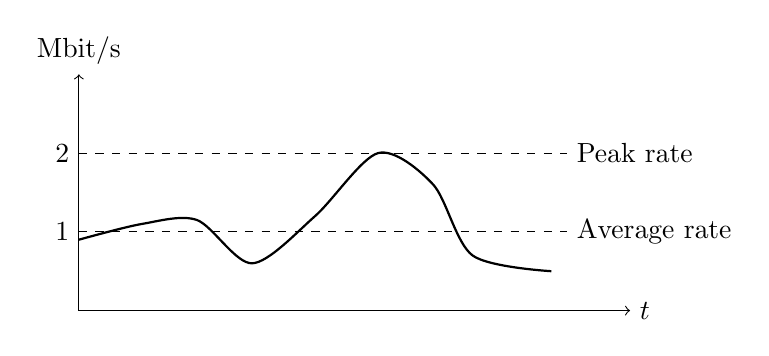
\begin{tikzpicture}[scale=1]

		% Axes
		\draw[->] (0,0) -- (7,0) node[right] {$t$};
		\draw[->] (0,0) -- (0,3) node[above] {Mbit/s};

		% Dashed reference lines
		\draw[dashed] (0,2) -- (6.2,2) node[right] {Peak rate};
		\draw[dashed] (0,1) -- (6.2,1) node[right] {Average rate};

		% Labels on y-axis
		\node[left] at (0,1) {1};
		\node[left] at (0,2) {2};

		% Traffic curve
		\draw[thick, smooth]
		plot coordinates {
		(0,0.9)
		(0.8,1.1)
		(1.5,1.15)
		(2.2,0.6)
		(3.0,1.2)
		(3.8,2.0)
		(4.5,1.6)
		(5.0,0.7)
		(6.0,0.5)
		};

	\end{tikzpicture}
	\caption{Esempio di traffico con bitrate variabile}
\end{figure}\noindent
In questo esempio vi sono diverse sorgenti, con bitrate massimo di $2 Mbit/s$ e bit rate medio di $1 Mbit/s$, che condividono un canale con capacità di $100Mbit/s$.
Ci sono diverse possibilità per multiplexare questi flussi:
\begin{itemize}
	\item 50 sorgenti: nessun multiplexing statistico, nessuna perdita di pacchetti, ma capacità del canale sottoutilizzata (in media il 50\% della capacità è inutilizzata)
	\item 100 sorgenti: multiplexing statistico, capacità del canale ben utilizzata, ma rischio di perdita di pacchetti quando il traffico totale supera i $100 Mbit/s$ (probabilità di perdita dipende dalla distribuzione del traffico)
\end{itemize}
\subsection{Code Division Multiplexing}
Particolarmente utile nelle reti wireless. 
Prevede l'utilizzo di una stazione di trasmissione che invia un segnale di sincronizzazione (pilot signal) a cui tutte le sorgenti si sincronizzano, e l'assegnazione di un codice unico a ogni sorgente.
\begin{enumerate}
	\item Il segnale $S_i$ viene moltiplicato per un codice $C_i$, generando la \textbf{sequenza di chip}.
	\item Tutti i segnali vengono sommati e trasmessi insieme.
	\item Il ricevitore, conoscendo il codice $C_i$ della sorgente che vuole ricevere, moltiplica il segnale ricevuto per $C_i$ e utilizza un filtro per estrarre il segnale $S_i$ originale.
\end{enumerate}

\begin{figure}[H]
\centering
\begin{tikzpicture}[>=Stealth, font=\footnotesize, line join=round]
% Asse principale
\draw[->, thick] (0,0) -- (15.2,0);

% Livelli riferimento per segnale in alto
\node[left] at (0.5,1.6) {+1};
\node[left] at (0.5,0.4) {-1};

% Segnale S_i (alto sinistra)
\draw[thick] (0.6,0.4) -- (0.6,1.6) -- (3.8,1.6) -- (3.8,0.4) -- (6.4,0.4) -- (6.4,1.6);
\node at (2.2,1.85) {1};
\node at (5.1,0.95) {0};
\node at (2.8,-0.9) {Signal $S_i$};

% Nodo di moltiplicazione
\node[draw, circle, minimum size=0.9cm, thick] (mul) at (7.6,0) {};
\draw[thick] (7.25,-0.35) -- (7.95,0.35);
\draw[thick] (7.25,0.35) -- (7.95,-0.35);


% Livelli riferimento per codice in basso
\node[left] at (5.9,-1.45) {+1};
\node[left] at (5.9,-2.45) {-1};

% Codice C_i (basso)
\draw[thick] (6.0,-2.45) -- (6.0,-1.45) -- (6.35,-1.45) -- (6.35,-2.45)
						 -- (6.8,-2.45) -- (6.8,-1.45) -- (7.2,-1.45) -- (7.2,-2.45)
						 -- (7.65,-2.45) -- (7.65,-1.45) -- (8.0,-1.45) -- (8.0,-2.45)
						 -- (8.35,-2.45) -- (8.35,-1.45) -- (8.75,-1.45) -- (8.75,-2.45)
						 -- (9.0,-2.45);

% Marcature tratteggiate chip
\foreach \x in {6.18,6.52,6.95,7.38,7.82,8.18,8.55} {
	\draw[densely dashed] (\x,-1.45) -- (\x,-2.45);
}

\node at (4.9,-2.0) {Code $C_i$};
\draw[->, thick] (7.6,-1.45) -- (mul.south);

% Sequenza trasmessa (alto destra)
\draw[thick] (8.6,1.6) -- (8.6,0.4) -- (9.0,0.4) -- (9.0,1.6)
						 -- (9.35,1.6) -- (9.35,0.4) -- (9.8,0.4) -- (9.8,1.6)
						 -- (10.2,1.6) -- (10.2,0.4) -- (10.55,0.4) -- (10.55,1.6)
						 -- (10.9,1.6) -- (10.9,0.4) -- (11.35,0.4) -- (11.35,1.6)
						 -- (11.75,1.6) -- (11.75,0.4) -- (12.1,0.4) -- (12.1,1.6)
						 -- (12.45,1.6) -- (12.45,0.4) -- (12.9,0.4) -- (12.9,1.6)
						 -- (13.2,1.6) -- (13.2,0.4) -- (13.7,0.4) -- (13.7,1.6)
						 -- (14.0,1.6);

\foreach \x in {8.75,9.15,9.55,9.95,10.35,10.75,11.15,11.55,11.95,12.35,12.75,13.15,13.55} {
	\draw[densely dashed] (\x,0.4) -- (\x,1.6);
}

\node at (12.0,-0.9) {Transmitted Sequence};
\end{tikzpicture}
\caption{CDM: moltiplicazione del segnale $S_i$ con il codice $C_i$ e generazione della sequenza trasmessa}
\end{figure}
Una proprietà fondamentale è che i codici $C_i$ devono essere ortogonali tra loro, ovvero $C_i \cdot C_j = 0$ per $i \neq j$, in modo da evitare interferenze reciproche.
\section{Accesso multiplo}

L'accesso multiplo riguarda la condivisione di un mezzo trasmissivo \emph{condiviso} tra più sorgenti trasmittenti in maniera concorrente (tipico scenario wireless).
Diverse sorgente sono connesse allo stesso mezzo di trasmissione e devono coordinare le loro trasmissioni per evitare collisioni e garantire un accesso equo al canale.

\begin{figure}[htbp]
\centering
\begin{tikzpicture}[
	>=Stealth,
	font=\footnotesize,
	box/.style={draw, thick, align=center, minimum width=3.1cm, minimum height=0.9cm},
	arrow/.style={->, thick}
]
\node[box, font=\bfseries] (ma) at (0,0) {Accesso multiplo};

\node[box] (chan) at (-4.8,-1.8) {Channelization\\FDMA / TDMA / CDMA};
\node[box] (rand) at (0,-1.8) {Random\\Aloha, CSMA};
\node[box] (ctrl) at (4.8,-1.8) {Controlled\\Reservation, Polling, Token passing};

\draw[arrow] (ma) -- (chan);
\draw[arrow] (ma) -- (rand);
\draw[arrow] (ma) -- (ctrl);
\end{tikzpicture}
\caption{Tassonomia semplificata delle tecniche di accesso multiplo}
\end{figure}
\noindent
Le \textbf{tecniche di canalizzazione} sono molto simili alle loro controparti di multiplazione, ma con l'obiettivo di coordinare l'accesso al canale condiviso piuttosto che combinare segnali da sorgenti diverse.
\begin{itemize}
	\item \textbf{(O)FDMA}: i carrier (e sotto-carrier) sono assegnati dinamicamente alle sorgenti che vogliono trasmettere, in modo da evitare interferenze.
	\item \textbf{TDMA}: i time slot sono assegnati dinamicamente alle sorgenti che vogliono trasmettere.
	\item \textbf{CDMA}: i segnali vengono moltiplicati per codici e vengono trasmessi da diverse fonti sullo stesso canale.
\end{itemize}
Le tecniche \textbf{random} e \textbf{controlled} condividono la capacità dividendo la risorsa temporale, ma in modo diverso da TDMA:
\begin{itemize}
	\item \textbf{Random}: accesso puramente concorrente al medium, in alcuni casi con meccanismi di rilevamento di collisioni e di elusione.
	\item \textbf{Controlled}: le sorgenti devono ottenere il permesso di trasmettere, c'è un meccanismo di sincronizzazione.
\end{itemize}

\section{Mezzi trasmissivi}
I mezzi trasmissivi si distinguono in:
\begin{itemize}
\item \textbf{Guidati}: La propagazione del segnale avviene per mezzo di un supporto fisico, come il doppino, il cavo coassiale, la fibra ottica;
\item \textbf{Radio}: propagazione in aria, soggetta a fading, attenuazioni atmosferiche e ostacoli. Permette di superare ostacoli fisici e di coprire grandi distanze,.
\end{itemize}
\subsection{Doppino}
Un doppino è costituito da due fili di rame isolati, attorcigliati tra loro per ridurre le interferenze elettromagnetiche.
Un paio di fili paralleli fungerebbero da antenna, dunque trasmetterebbe il segnale che porta e sarebbe soggetto a interferenze da parte di segnali esterni.
Essendo attorcigliati, una interferenza distruttiva viene generata e il segnale trasmesso viene preservato.
\begin{figure}[H]
\centering
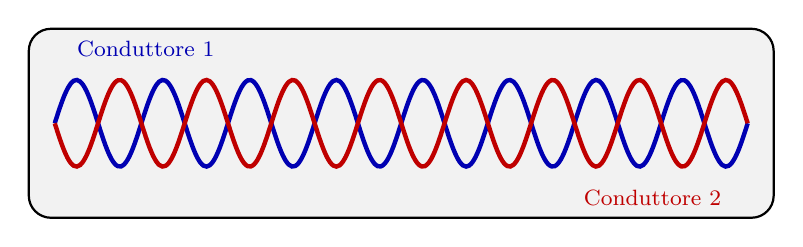
\begin{tikzpicture}[x=0.55cm,y=1cm,font=\footnotesize]
	% Guaina esterna
	\draw[rounded corners=8pt, thick, fill=gray!10] (-0.6,-1.2) rectangle (16.6,1.2);

	% I due conduttori intrecciati (vista laterale semplificata)
	\draw[line width=1.6pt, blue!70!black, samples=220, domain=0:16, smooth]
		plot (\x,{0.55*sin(180*\x)});
	\draw[line width=1.6pt, red!75!black, samples=220, domain=0:16, smooth]
		plot (\x,{-0.55*sin(180*\x)});

	% Etichette
	\node[blue!70!black] at (2.1,0.95) {Conduttore 1};
	\node[red!75!black]  at (13.8,-0.95) {Conduttore 2};
\end{tikzpicture}
\caption{Rappresentazione semplificata di un doppino intrecciato}
\end{figure}
Il caso tipico, tuttavia, presenta più coppie di fili attorcigliati, ognuna con una frequenza di attorcigliamento diversa, in modo da impedire disturbi reciproci tra coppie diverse.
I doppini vengono classificati in base alla categoria, che indica la frequenza massima supportata e la qualità del cavo (e.g., Cat 5, Cat 6, Cat 7).
\begin{figure}[H]
\centering
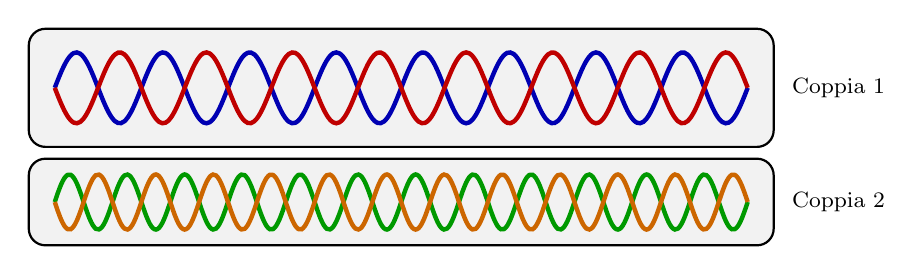
\begin{tikzpicture}[x=0.55cm,y=1cm,font=\footnotesize]

	% Coppia 1 (frequenza 1x)
	\draw[rounded corners=6pt, thick, fill=gray!10] (-0.6, 1.55) rectangle (16.6, 3.05);
	\draw[line width=1.6pt, blue!70!black, samples=220, domain=0:16, smooth]
		plot (\x,{2.3 + 0.45*sin(180*\x)});
	\draw[line width=1.6pt, red!75!black, samples=220, domain=0:16, smooth]
		plot (\x,{2.3 - 0.45*sin(180*\x)});
	\node[anchor=west] at (16.8, 2.3) {Coppia 1};

	% Coppia 2 (frequenza 1.5x)
	\draw[rounded corners=6pt, thick, fill=gray!10] (-0.6, 0.3) rectangle (16.6, 1.4);
	\draw[line width=1.6pt, green!60!black, samples=220, domain=0:16, smooth]
		plot (\x,{0.85 + 0.35*sin(270*\x)});
	\draw[line width=1.6pt, orange!80!black, samples=220, domain=0:16, smooth]
		plot (\x,{0.85 - 0.35*sin(270*\x)});
	\node[anchor=west] at (16.8, 0.85) {Coppia 2};
\end{tikzpicture}
\caption{Doppino con più coppie di fili attorcigliati, ognuna con una frequenza di attorcigliamento diversa}
\end{figure}
I doppini formano la base delle reti telefoniche e ADSL/VDSL.
Molto spesso i cavi utilizzati per questi scopi sono vecchi e non possono essere classificati in una delle categorie citate precedentemente.
La velocità di trasmissione in questi contesti è molto variabile.
\subsection{Fibre ottiche}

